\documentclass[11pt,a4paper]{article}

\usepackage[T1]{fontenc}
\usepackage[utf8]{inputenc}
\usepackage{charter}
\usepackage[a4paper,margin=1.15in]{geometry}
\usepackage{amsmath,amssymb}
\usepackage{graphicx}
\usepackage{booktabs}
\usepackage{tabularx}
\usepackage{enumitem}
\usepackage{xcolor}
\usepackage{fancyhdr}
\usepackage{titlesec}
\usepackage{caption}
\usepackage[hidelinks]{hyperref}

\setlength{\parindent}{0pt}
\setlength{\parskip}{0.55em}
\setlist{itemsep=0.25em,topsep=0.3em}
\captionsetup{font=small,labelfont=bf}

\newcommand{\key}[1]{\textcolor{blue}{\textbf{#1}}}

% a quoted line from the supervisor's review, with its section
\newenvironment{review}[1]
  {\par\smallskip\noindent\begin{minipage}{\linewidth}\begin{list}{}{\leftmargin=1.2em\rightmargin=1.2em}\item[]%
   \def\reviewsrc{#1}\small\itshape\color{black!80}}
  {\par\hfill\upshape\footnotesize --- Review, \reviewsrc\end{list}\end{minipage}\par\smallskip}

\pagestyle{fancy}
\fancyhf{}
\renewcommand{\headrulewidth}{0.4pt}
\renewcommand{\footrulewidth}{0.4pt}
\renewcommand{\sectionmark}[1]{\markright{\thesection\quad\MakeUppercase{#1}}}
\fancyhead[R]{\small\itshape\rightmark}
\fancyfoot[R]{\thepage}

\titleformat{\section}{\Large\bfseries}{\thesection}{1em}{}
\titleformat{\subsection}{\large\bfseries}{\thesubsection}{1em}{}

\begin{document}

\begin{titlepage}
\centering
\vspace*{2.2cm}
{\Large\textbf{ME303 - \textsc{Study Oriented Program}}\par}
\vspace{0.9cm}
{\Large BITS \textsc{Pilani}\par}
\vspace{0.3cm}
{\large \textsc{Department of CSIS}\par}
\vspace{1.4cm}
\rule{\linewidth}{0.8pt}\par\vspace{0.3cm}
{\huge\bfseries Response to Review: Stages A and B\par}
\vspace{0.3cm}
{\Large Is the problem real, and is reinforcement learning needed?\par}
\vspace{0.2cm}
\rule{\linewidth}{0.8pt}\par
\vspace{1.8cm}
\begin{flushleft}
\textit{Author:}\\
Chaitanya Goyal (ID: 2024A7PS0557P)\\[0.8em]
\textit{Supervisor:}\\
Prof. Avinash Gautam\\[0.8em]
\textit{In response to:}\\
``Value-Aware Adaptive Multi-Robot Exploration under Resource Constraints'', review report dated October 21, 2026\\
\vspace{2.4cm}
Date: November 2026
\end{flushleft}
\end{titlepage}

% ================================================================
\section{Summary}

The review asked for two things to be checked before any MARL work: whether the problem is real (Stage A), and whether a learned value estimate is possible and actually needs reinforcement learning (Stage B). Both are done. Each section below quotes the review's request, then says what I did and what came out.

\begin{itemize}
  \item \key{Stage A: the problem is real, under a condition.} In 1,432 of 1,440 runs, the best moment to stop came before the map was finished. Exploring until done lost 11.4\% of the map's value on average and up to 44.6\% in one setting, and 36\% of all driving happened after the best stop. But the loss shrinks to 1--2\% when driving is cheap, so it matters only when motion or messaging is expensive.
  \item \key{Stage B: the RL-style target is needed; a big model is not.} Every model trained with fitted Q-iteration beat every model trained by plain regression on hindsight values, most clearly in the worst case (9.9--13.0\% of the map lost versus 30.4--39.0\%). The choice of model mattered little: even a linear model works.
\end{itemize}

Everything here can be reproduced from the project repository:\\
\url{https://github.com/dev-goyal-chaitanya/marl-simulations}\\
(scripts \texttt{week1\_problem\_size.py} and \texttt{week2\_models.py}).

% ================================================================
\section{Setup Used for Both Stages}

\begin{itemize}
  \item \textbf{World:} random indoor buildings (rooms, doors, furniture) on $32\times32$, $48\times48$ and $64\times64$ grids. Robots see 4 cells around them, and walls block the view.
  \item \textbf{Robots:} 2, 4, 6 or 8 robots. They move with a fixed nearest-frontier rule, so only the stopping decision changes between methods.
  \item \textbf{Score of one cycle (6 robot steps):} new cells seen $-\,2\times$robot steps $-\,c_{\text{comm}} N(N-1) - 2$, with $c_{\text{comm}} = 0.05, 0.2, 0.6$ for cheap, medium and expensive messaging.
  \item \textbf{Best stop in hindsight:} $T^* = \arg\max_T V(T)$, where $V(T)$ is the total score after $T$ cycles. It is used only as the 100\% reference.
  \item \textbf{Test set:} 36 settings (4 team sizes $\times$ 3 map sizes $\times$ 3 message costs), 40 maps each, never seen in training.
\end{itemize}

% ================================================================
\section{Stage A: Is the Problem Real?}

\subsection{What the review asked}

\begin{review}{Sec.~9.1}
Initially, no MARL is required. Generate a large number of complete exploration trajectories and calculate the hindsight-optimal stopping point $T^* = \arg\max_T V(T)$. The first empirical question should be: How much mission value is actually lost by continuing exploration until conventional completion? This should be evaluated across many maps, team sizes, and cost regimes. If the difference between conventional termination and value-aware termination is negligible, there is little reason to develop a sophisticated learning method. If the difference is substantial and systematic, we have established the practical significance of the research problem.
\end{review}

\begin{review}{Sec.~17, item 3}
Generate a sufficiently large collection of complete exploration trajectories and examine the distribution of hindsight-optimal stopping points under different maps, team sizes, and cost regimes.
\end{review}

\subsection{What I did}

No learning at all. I ran 480 complete explorations (12 team/map combinations $\times$ 40 maps) all the way until no frontier was left, and scored each one under the three message costs, giving 1,440 scored runs. For each run I found the best stop $T^*$ and compared it with ``explore until done'' on three things:
\begin{itemize}
  \item \textbf{value lost:} $V(T^*) - V(T_{\text{end}})$, as a percentage of the cells the full exploration revealed;
  \item \textbf{wasted driving:} the share of all robot steps taken after $T^*$;
  \item \textbf{where $T^*$ falls:} $T^*$ as a fraction of the full mission length.
\end{itemize}

\subsection{What came out}

\begin{table}[h]
\centering
\small
\begin{tabular}{lccc}
\toprule
Team size & Cheap messages & Medium & Expensive \\
\midrule
2 robots & 9.3 & 9.6 & 10.3 \\
4 robots & 6.1 & 7.2 & 10.6 \\
6 robots & 6.3 & 8.8 & 18.5 \\
8 robots & 5.8 & 10.8 & 33.8 \\
\bottomrule
\end{tabular}
\caption{Value lost by exploring until done (\% of map), averaged over the three map sizes, 40 maps each.}
\end{table}

\begin{figure}[h]
\centering
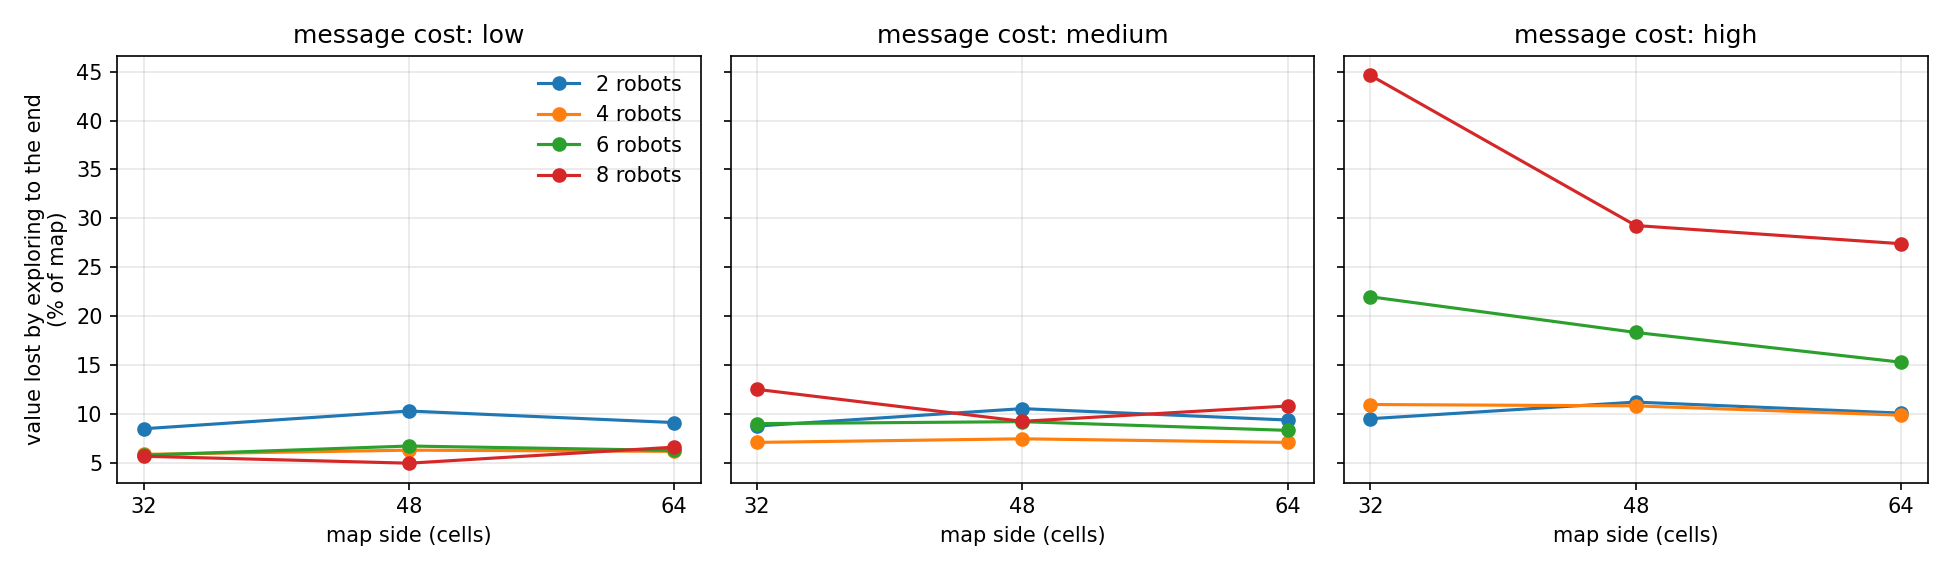
\includegraphics[width=\linewidth]{figures/week1_value_lost.png}
\caption{The same loss by map size. Each panel is one message cost; each line is one team size.}
\end{figure}

\begin{itemize}
  \item \textbf{Across all 36 settings}, exploring until done lost \key{11.4\% of the map's value} on average (lowest 5.0\%, highest 44.6\%). \key{36\%} of all driving happened after the best stop.
  \item \textbf{The loss is systematic, not random:} it grows with team size (8 robots: 16.8\% versus 4 robots: 8.0\%) and with message cost (expensive: 18.3\% versus cheap: 6.9\%).
\end{itemize}

\textbf{Where the best stop falls} (the distribution asked for in item 3):

\begin{table}[h]
\centering
\small
\begin{tabular}{lcccc}
\toprule
Message cost & Median $T^*$ & 10th--90th pct. & $T^*$ at the end & $T^*$ at cycle 0 \\
\midrule
Cheap & 70\% & 47--90\% & 6 of 480 & 0 \\
Medium & 65\% & 41--84\% & 1 of 480 & 0 \\
Expensive & 50\% & 13--78\% & 1 of 480 & 30 of 480 \\
\bottomrule
\end{tabular}
\caption{$T^*$ as a fraction of the full mission length.}
\end{table}

\begin{figure}[h]
\centering
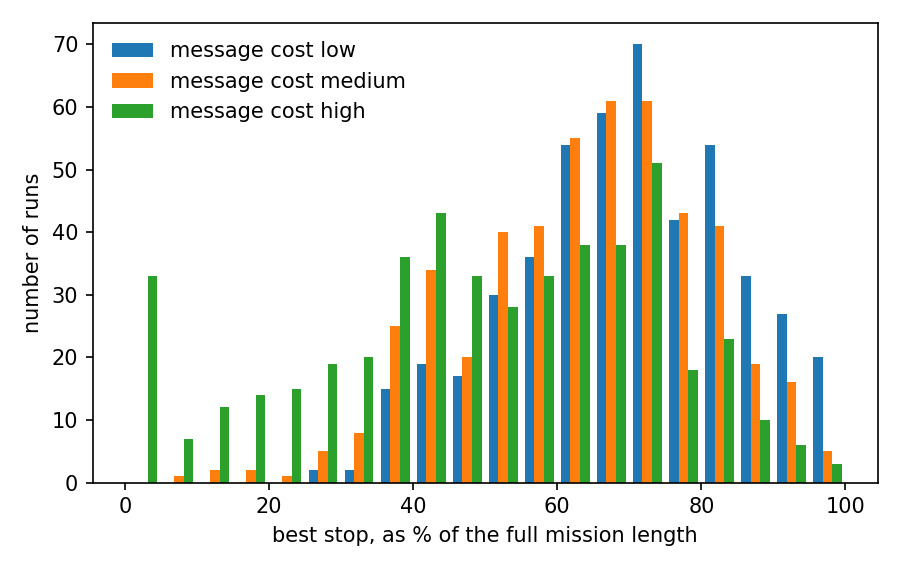
\includegraphics[width=0.7\linewidth]{figures/week1_where_best_stop_falls.png}
\caption{Histogram of $T^*$ as a percentage of the full mission, by message cost.}
\end{figure}

So in almost every run (1,432 of 1,440) it was better to stop before the map was finished, and the best moment moves earlier as costs rise. In 30 expensive-messaging runs, not exploring at all would have scored best, because the cost of a large team talking to itself outweighs any map gained.

\subsection{The condition: it depends on the price of driving}

All of the above uses a cost of 2 per robot step. Re-scoring the same runs at medium message cost with other prices:

\begin{table}[h]
\centering
\small
\begin{tabular}{ccc}
\toprule
Cost per robot step & Value lost (\% of map) & Driving after the best stop \\
\midrule
0.5 & 1.0 & 4.8\% \\
1 & 2.2 & 9.6\% \\
2 (default) & 9.1 & 33.1\% \\
3 & 27.3 & 67.8\% \\
\bottomrule
\end{tabular}
\caption{The size of the problem depends on how expensive driving is.}
\end{table}

\textbf{Answer to the review's question:} the difference is \emph{substantial and systematic} when motion or communication is expensive, and close to \emph{negligible} when they are cheap. The next step is to fix realistic cost values (or present the whole sweep as a trade-off curve, as the review's Section 11 suggests).

% ================================================================
\section{Stage B: Can the Value Be Learned, and Is RL Needed?}

\subsection{What the review asked}

\begin{review}{Sec.~9.2}
Before MARL, evaluate whether continuation value can be estimated using relatively simple models. Possible comparisons include: linear regression; decision trees/random forests; ExtraTrees; multilayer perceptrons; CNN-based map encoders; graph neural networks; recurrent models. If a simple model solves the problem effectively, that is scientifically informative and should not be hidden.
\end{review}

\begin{review}{Sec.~17, item 4}
Compare simple regression/value-estimation models against fitted Q-iteration. Establish whether reinforcement learning is actually necessary for the stopping component.
\end{review}

\begin{review}{Sec.~7.1, RQ1}
Can the remaining marginal value of multi-robot exploration be estimated online from partial observations? [\dots] The learned estimate $\hat V(b_t)$ should be compared against the continuation value available retrospectively from complete trajectories.
\end{review}

\subsection{What I did}

I kept everything else fixed: the same 7 team-level features (all ratios, such as map known and expected gain per unit cost), the same 300 training runs (2 robots, $32\times32$), each re-scored under 4 random cost settings. Only two things changed:

\begin{itemize}
  \item \textbf{How the training target is built.}
  \begin{itemize}
    \item \emph{Hindsight regression (plain supervised learning):} the target at each moment is the best value still achievable from there, read off the finished run. One fit.
    \item \emph{Fitted Q-iteration (RL-style):} the target is this cycle's score plus the model's own estimate for the next moment (counted as 0 if negative, since the team could stop there). Refit 25 times.
  \end{itemize}
  \item \textbf{Which model learns it:} linear regression, random forest, ExtraTrees, and a small neural network (MLP, two layers of 64).
\end{itemize}

Each version stops at the first cycle where its estimate is $\le 0$. All were tested on the 36 settings without retraining.

\subsection{What came out}

\begin{table}[h]
\centering
\small
\begin{tabular}{llccc}
\toprule
Training target & Model & Avg value lost & Worst setting & Settings $<$50\% \\
\midrule
\textbf{Fitted Q-iteration} & \textbf{ExtraTrees} & \textbf{3.6} & \textbf{9.9} & \textbf{1} \\
Fitted Q-iteration & random forest & 3.7 & 10.3 & 1 \\
Fitted Q-iteration & linear & 3.5 & 13.0 & 4 \\
Fitted Q-iteration & MLP & 4.8 & 12.1 & 1 \\
Hindsight regression & linear & 6.7 & 30.4 & 6 \\
Hindsight regression & MLP & 5.4 & 37.4 & 5 \\
Hindsight regression & random forest & 9.0 & 35.7 & 8 \\
Hindsight regression & ExtraTrees & 9.6 & 39.0 & 8 \\
\midrule
\multicolumn{2}{l}{Coverage threshold (tuned), for reference} & 4.7 & 25.3 & 5 \\
\bottomrule
\end{tabular}
\caption{Value lost versus the best stop in hindsight (\% of map) over 36 unseen settings. ``Settings $<$50\%'' counts settings where a rule kept less than half of the best value.}
\end{table}

\begin{figure}[h]
\centering
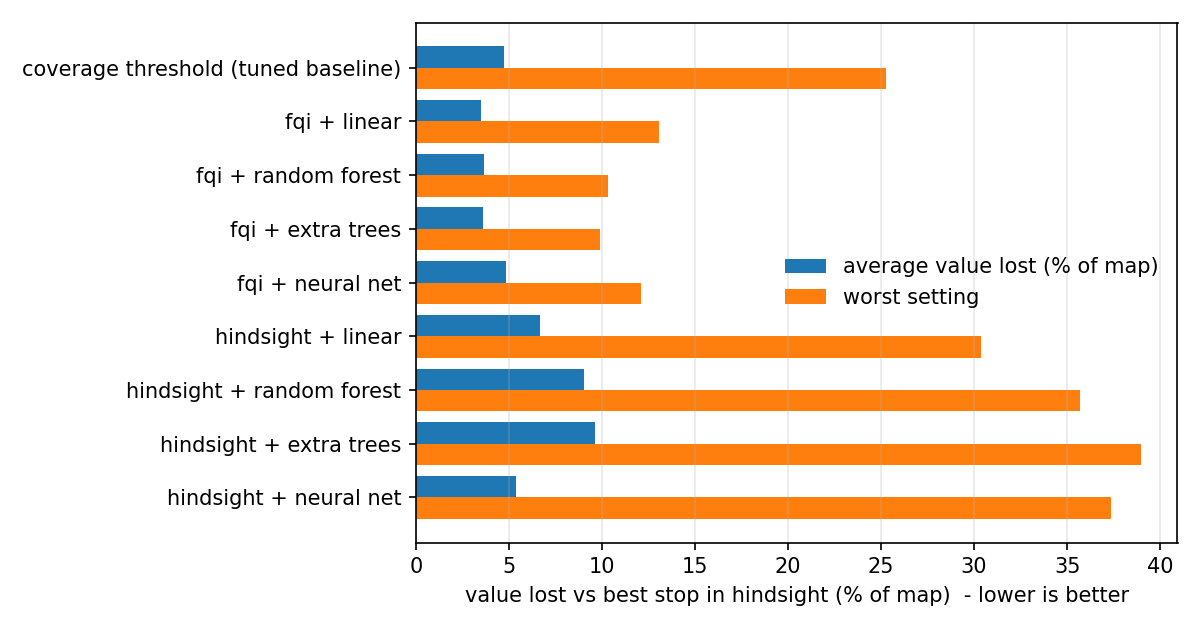
\includegraphics[width=0.82\linewidth]{figures/week2_models.png}
\caption{Average value lost (blue) and the worst setting (orange) for each version.}
\end{figure}

\begin{enumerate}
  \item \key{The target matters, the model does not.} Every fitted Q-iteration version beats every hindsight-regression version, most clearly in the worst case (9.9--13.0\% against 30.4--39.0\%).
  \item \key{A simple model is enough.} Linear regression inside fitted Q-iteration is nearly as good as ExtraTrees; the MLP adds nothing. As the review asks, this is reported and not hidden.
  \item \key{The value can be estimated online (RQ1).} The fitted Q-iteration estimate from partial observations has a correlation of 0.88 with the true remaining value from complete runs, and gets its sign (``still worth continuing?'') right 89\% of the time on 100 test maps.
\end{enumerate}

\subsection{Why hindsight regression fails}

The hindsight target says ``this much value was still possible'', but reaching it requires stopping at exactly the right later moment, which needs the future. So the targets are biased upward, the model overvalues continuing, and the team stops too late. This is the perfect-foresight bias known in regression-based optimal stopping (Longstaff and Schwartz, 2001). The fitted Q-iteration target only credits what the learned rule itself can achieve.

\subsection{Answer to the review's question}

\begin{review}{Sec.~18, question 2}
Why does the problem require reinforcement learning or MARL rather than continuation-value regression combined with an existing exploration policy?
\end{review}

For the stopping component, the answer is precise: \textbf{the reinforcement-learning-style target is needed, but a large learner is not}. Fitted Q-iteration is itself regression repeated with a bootstrapped target, and with that target even a linear model works. Plain regression on hindsight continuation values is not enough. \textbf{MARL is not needed for stopping alone}; following the review, it should only enter if adaptive team size (Stage D) shows that the allocation and exploration decisions need to be learned together.

% ================================================================
\section{What Is Still Missing}

\begin{itemize}
  \item \textbf{Model families from Sec.~9.2 not yet tested:} CNN map encoders, graph neural networks and recurrent models.
  \item \textbf{One building style} (rooms with furniture); maze, warehouse and cluttered maps still to come.
  \item \textbf{One training seed} per model; 5 seeds are planned.
  \item \textbf{Assumed costs}, not measured from real robots.
  \item \textbf{Known failure:} with 2 robots on $48\times48$ and $64\times64$ maps the learned stop sometimes stops 20--33 cycles early; not yet diagnosed.
\end{itemize}

% ================================================================
\section{Next Steps}

Following Sec.~17 of the review:
\begin{enumerate}
  \item Realistic costs, or the full cost sweep presented as a trade-off curve.
  \item Stage C: add stopping rules based on Amorín et al.\ (2019), Luperto et al.\ (2026) and PRoID (2026) to the benchmark.
  \item Stage D: generalise the action from stop/continue to $N^{\text{active}}_t \in \{0,\dots,N\}$ and test whether shrinking the team gives a real advantage.
  \item Fix the generalisation tests (environment, scale, team size, communication) before training the final model.
\end{enumerate}

\end{document}
